\documentclass{article}
\usepackage{graphicx}
\usepackage{hyperref}
\hypersetup{
    colorlinks=true,
    linkcolor=blue,
    filecolor=magenta,      
    urlcolor=red,
}
\usepackage{listings} % nice code layout
\usepackage[section]{placeins}
\usepackage{xcolor}
\usepackage[utf8]{inputenc}
\lstset{language = Verilog}
\graphicspath{ {./images/} }

\author{Justin Bui}
\title{Simple Adder and Subtractor Testing with UVM}

\begin{document}

\maketitle
\newpage

\tableofcontents
\newpage

\section{Introduction}
This document discusses the adder/subtractor circuit built to help introduce the concepts of UVM. UVM, or the Universay Verification Methodology is a testing and validation platform which allows for the design and development of testbenches and more advanced simulations of our SystemVerilog designs. This project's aim is to briefly introduce the basics of UVM, as well as develop a simple testbench based on the \href{https://www.edaplayground.com/x/296}{UVM Hello World Example}. This project has been completely written and tested using the \textbf{EDA Playground}.

The code for my UVM Adder/Subtractor can be found \href{https://www.edaplayground.com/x/2_RZ}{here}.


\section{Project Description}
The Adder and Subtractor project is a simple implementation of an 8 bit circuit designed to introduce the concepts of UVM testing and testbench development. In order to implement the testbench prototype provided by the \textbf{Hello World} example, I had to modify the number of interface signals (we know them as ports when using Vivado). For this project, I use the following signals:
\begin{center}
	\begin{itemize}
		\item \textbf{clock} - 1 bit clock
		\item \textbf{reset} - 1 bit reset
		\item \textbf{opp} - 1 bit operator
		\item \textbf{numA} - 8 bit number A
		\item \textbf{numB} - 8 bit number B
		\item \textbf{sum} - 8 bit output
		\item \textbf{cout} - 1 bit carry out
	\end{itemize}
\end{center}

The logic for this circuit is pretty simple, and can be implemented using one \textbf{If-Else} statement. The operation values are defined in the project requirements. A value of \textbf{0} for the operator results in an \textbf{add} operation, and a value of \textbf{1} testults in a subtraction operation. The system performs the operation on the positive clock edge. In order to account for the carry bit, I make use of an internal sum value, \textbf{isum}, which is 9 bits long to allow for the storage of the carry out. After the caluclation is performed, values of sum and cout are updated. All of the signals are then printed using a system print.

\section{Design Validation}
The strenght of UVM is in the ability to develop test benches, allowing us to determine whether the functionality of our device matches our expectations. The breakdown of the UVM testbench is well documented, and a quite complex. Test benches allow for multiple environments, sequences, and drivers, however, for our introductory project, we only make use of one driver, sequence and environment. I have written by sequence to generate 3 random signals, one for the operator bit, and two for the 8 bit numbers \textbf{numA} and \textbf{numB}. I have programmed the device to run through 25 loops, the results of which are printed in the log file when the program is run.

The Log at the bottom of the screen will print out an "overview" which essentially sumarizes the UVM outputs. Figure \ref{fig:over} below shows the UVM outputs for the simulation I ran prior to submission of this document. Figure \ref{fig:results} shows the results for the 25 simulated runs. 

\begin{center}
	\begin{figure}[h!]
		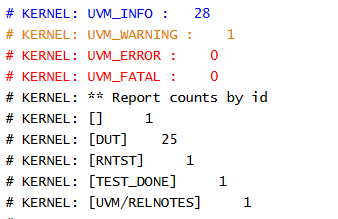
\includegraphics{report.png}
		\caption{UVM Outputs}
		\label{fig:over}
	\end{figure}
\end{center}

In order to verify the operating is working correctly, I checked the calculated values by hand. Although this is a slow method, I was able to verify the operation of the adder/subtractor. It is likely that, should time permit in the future, the testing capabilities will be expanded to include more in-depth test coverage, as well as test validation.

\begin{center}
	\begin{figure}[h!]
		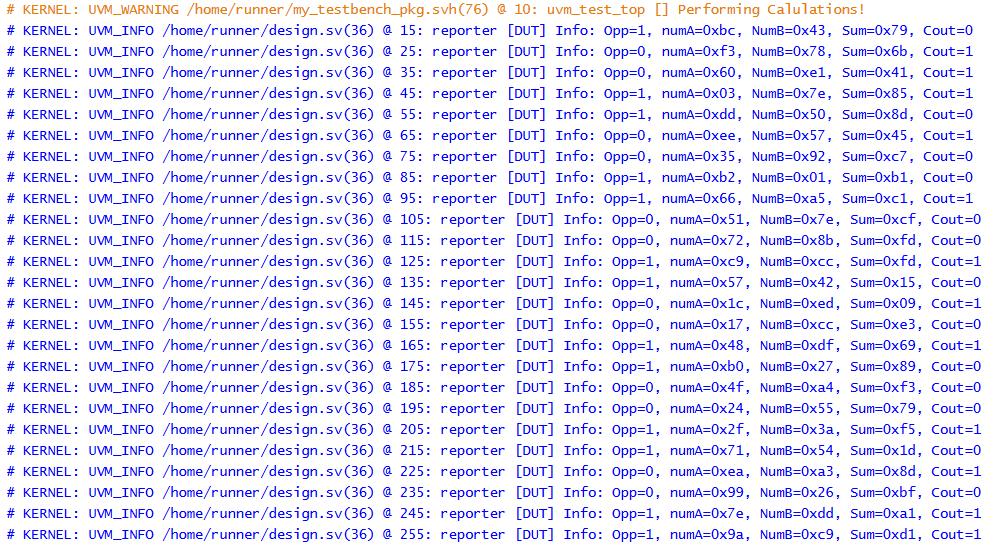
\includegraphics[width=.9\textwidth]{results.png}
		\caption{Results}
		\label{fig:results}
	\end{figure}
\end{center}


\end{document}